%
% DS 5220 Final
%
\documentclass[11pt]{article}

%
% Packages
%
\usepackage{amsmath}
\usepackage{amssymb}
\usepackage{amsthm}
\usepackage{clrscode3e}
\usepackage{enumerate}
\usepackage{graphicx}
\usepackage[table]{xcolor}% http://ctan.org/pkg/xcolor
\usepackage{caption}
\usepackage{subcaption}


%
% Package settings
%

%% begin.rcode setup, include=FALSE
% library(knitr)
%
% opts_chunk$set(fig.path='figure/latex-', cache.path='cache/latex-')
%% end.rcode

%
% Document Settings
%
\setlength{\parskip}{1pc}
\setlength{\parindent}{0pt}
\setlength{\topmargin}{-3pc}
\setlength{\textheight}{9.5in}
\setlength{\oddsidemargin}{0pc}
\setlength{\evensidemargin}{0pc}
\setlength{\textwidth}{6.5in}


\title{Quick, Draw! Image Classification}
\author{Group 3}

%
% Image directory location
%
\graphicspath{ {./imgs/} }

\begin{document}

\maketitle

\section{Introduction}

Many recent industry innovations have included neural networks. An
important research area within neural networks has been image classification.
One of the best techniques to classify images is Convolutional Neural
Networks (CNN). We have sought to better understand industry best practices
by exploring different image classification techniques with neural networks.
Our exploration starts by manually performing image classification and
noting the level of human accuracy. We then use a fully connected neural
network to perform image classification before implementing a CNN. We
implemented options for tuning and debugging the neural network while
implementing each method during our process. We were able to develop an
intuition for image classification best practices using neural networks
after our research.

Many supervised machine learning methods often differ from those employed 
when constructing neural networks. These supervised machine learning
methods, such as logistic regression or decision tree classification,
require feature engineering to successfully classify an image. Models
requiring feature engineering rely on considerable effort by subject matter
experts to achieve reasonable accuracy. Neural networks allow for an
approach which does not require feature engineering to achieve similar or
better accuracy. Industry engineering efforts regarding feature engineering
can be shifted to neural networks  in some cases such as image
classification. Moreover, the availability of cheap computing resources
sped up a shift towards the use of neural networks.

When considering modeling approaches, we examine both fully connected and 
convolutional neural networks. A fully connected neural network is known to 
be inefficient at classifying large images. These inefficiencies in a fully 
connected neural network partly arise because every neuron in the $\ell-1$
layer must be connected to the $\ell$th layer. This requires a series
of matrix multiplications and additions across each layer $\ell$.
Alternatively, a CNN allows for more efficient computations by: (1) efficient
and automatic feature generation using local connectivity and parameter
sharing of convolution operations, (2) dimensionality reduction using pooling
layers. In this project, we attempt to understand these topics in depth
from an empirical stanpoint in relation to image classification using
Google's ``Quick, Draw!'' dataset.

\section{Methods}

Our methodology consists of reviewing statistical methodology, presenting
theoretically informed hypotheses, and providing an overview of our data.

\subsection{Overview of Statistical Modeling Techniques}

We use human classification, fully connected neural networks,
and a Convolutional Neural Network (CNN). We use more detail to
describe techniques not covered during the course.

\subsubsection{Understanding the Loss Function}

Most modern neural networks are trained using maximum likelihood. This
means that the cost function is the negative log-likelihood, also
described as the cross-entropy between the training data and the model
distribution \cite{Goodfellow-et-al-2016}. In our use case, we are interested
in correctly classifying 10 categories of drawings. Our output layer
uses a Softmax function to represent the probability distribution over
$k$ different classes. Given features $h$, weights $W$, and bias $b$, a
linear layer first predicts unnormalized log probabilities:
\begin{equation}
  z = W^Th + b 
\end{equation}

where $z_i = \log \tilde{P}(y = i | x)$. The softmax function can then
exponentiate and normalize $z$ to obtain the desired $\hat{y}$. The
softmax function is given by
\begin{equation}
  \func{softmax}(z)_i = \frac{\exp(z_i)}{\sum_j \exp(z_j)}.
\end{equation}

As a cost function, we wish to maximize
$\log P(y=i; z) = \log \func{softmax}(z)_i$. We can do this formally as
\begin{equation}
  \log \func{softmax}(z)_i = z_i - \log \sum_j \exp(z_j).
\end{equation}

which gives us the intuition for a single example. Overall, we want to learn
parameters that drive the softmax to predict the fraction of counts of each
outcome observed in the training set \cite{Goodfellow-et-al-2016}:
\begin{equation}
  \func{softmax}(z(x;\theta))_i \approx \frac{\sum_{j=1}^m 1_{y^{(j)} = i,
      x^{(j)} = x}}{\sum_{j=1}^m 1_{x^{(j)} = x}}.
\end{equation}

This is how the $\func{categorical\_crossetropy}(\text{y\_true}, \text{y\_pred})$ function is constructed in Keras \cite{chollet2015keras} as well as the
$\func{softmax\_cross\_entropy\_with\_logits\_v2}(\text{labels}, \text{logits})$ in Tensorflow \cite{tensorflow2015-whitepaper}. 

\subsubsection{Understanding the Optimization Technique}

This course discussed optimization algorithms such as Stochastic Gradient
Descent ($m =1$) and Batch Gradient Descent ($m=n \text{ obs.}$). Current
best practices for Neural Networks recommend Mini-Batch Gradient Descent
($m = c \text{ batch size}$). In practice, we use the Adam optimization
algorithm due to faster computation time. The Adam optimization algorithm
is able to achieve a speedup due to its combination of two other techniques.

The Adam optimization algorithm takes an exponentially weighted average of
the gradients, a technique called momentum, and then uses that gradient to
update your weights. Secondly, we also want to slow down gradient descent in
the horizontal direction with a technique called RMSprop to reduce
oscillations from batch gradient descent. The Adam optimization method is
combining momentum and RMSprop to perform gradient descent more quickly
\cite{DeepLear51:online}.

\subsubsection{Convolutional Neural Network (CNN)}

Convolutional networks, also known as convolutional neural networks(CNNs),
are a specialized kind of neural network for processing data that has a
known grid-like topology. Convolutional networks have been tremendously
successful in practical applications. The name “convolutional neural network”
indicates that the network employs a mathematical operation called
convolution. Convolution is a specialized kind of linear operation.
Convolutional networks are simply neural networks that use convolution
in place of general matrix multiplication in at least one of their layers. See
Figure \ref{fig:CNN} in the Appendix for a visual representation of a CNN.

CNN architectures are usually composed of the building blocks as described
below:

\begin{enumerate}
\item \textbf{Convolution:} The convolution operation helps to extract features
  from the input image. The first argument is often referred
  to as the input. The second is a feature detector (kernel) and
  the output is the feature map. The convolution operation takes the dot
  product of the feature detector and the input. Each convolution operation
  focuses on a subset of an image. This approach allows for parameter
  sharing which leads to a reduction in parameters relative to a
  fully connected neural network. The advantage 
  is that we can have a deeper network with fewer parameters.

  \begin{itemize}
  \item \textbf{Strides:} Stride is the number of pixels jumps between
    each convolution operation performed on the input matrix. When the stride
    is 1 then we move the filters to 1 pixel at a time. Increasing the stride
    parameter reduces the output volume of the convolution since the jumps
    are larger.
  \item \textbf{Padding:} Padding helps to detect features present at the
    border by adding a dummy values around the edge. Since convolution
    operations collect most information from the center of the image, adding
    padding allows the border pixels to be weighed more during the convolution
    operation.
  \end{itemize}

  See Figure \ref{fig:CNNStridePad} in the Appendix for an example of Stride
  and Padding.

\item \textbf{Pooling Layer:} Pooling layers section helps to reduce the
  number of parameters when the images are too large. Spatial pooling
  (subsampling or downsampling) reduces the dimensionality of each map,
  retaining important information. These can be of different types:
  (1) Max Pooling - takes the largest element (most important feature)
  from the rectified feature map (2) Average Pooling - averages all the
  pixel values (3) Sum Pooling. sum of all pixels values. See figure
  \ref{fig:CNNPooling} for a visualization of a Pooling Layer.

\item \textbf{Fully Connected (FC) Layer:} The FC layer flattens our
  matrix into vector and feeds it into a fully connected neural network layer.
  \end{enumerate}

\subsection{Hypotheses}

We have generated the following hypotheses based on theoretical
expectations expressed in the literature \cite{Goodfellow-et-al-2016,
  DeepLear51:online}. Performance is effected by both the model and
data \cite{DeepLear51:online} so our hypotheses pertain to both effects.

\subsubsection{Addressing model component of performance}

\begin{itemize}
  \item[$H1_a$] Fully Connected Neural Network will struggle to get reasonable
    accuracy.
  \item[$H2_a$] CNN should perform better than fully connected neural network.
  \end{itemize}

\subsubsection{Addressing data component of performance}

\begin{itemize}
\item[$H3_a$] Small amounts of data will lead to overfitting.
\item[$H4_a$] Imbalanced class prediction can be improved using data
  augmentation.
\item[$H5_a$] Addition of a category to the trained model will reduce the
  performance of the model.
\item[$H6_a$] Adding more training data will improve the performance of the
  model.
\end{itemize}

\subsection{Data}

Google originally collected the data from users by explicitly asking users to
draw objects like forks, hotdogs, etc \cite{QuickDra91:online}. The original
dataset is 70 GB in size but Google also provides a simplified version of the
dataset- consisting only of the final images \cite{googlecr61:online}. We
used these '.npy' files to train all of our models. These numpy bitmap files
consist of more than 100,000 rows each and 784
features, since they are basically $28 \times 28$ images. Samples of these
images are shown in Figure \ref{fig:quickImages}. The subset of this
dataset sampled varies from experiment to experiment. More details can be
found in the experiments mentioned below.

\begin{figure}[h]
  \begin{center}
    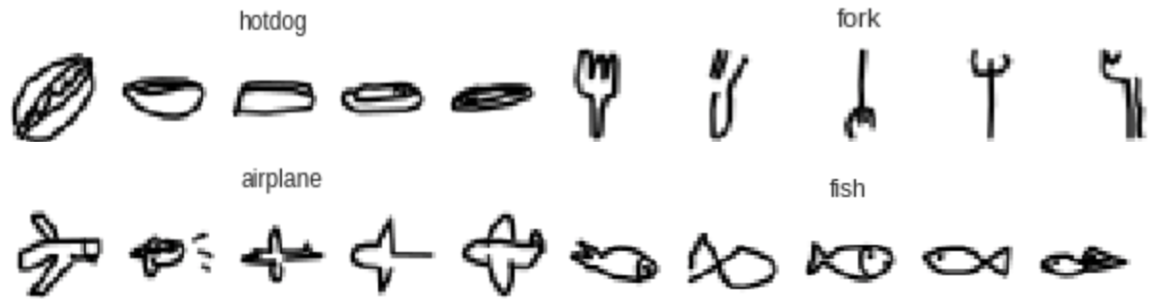
\includegraphics[scale=0.5]{fig1}
  \end{center}
  \caption{Sample images from Quick, Draw! dataset}
  \label{fig:quickImages}
\end{figure}

Our analysis required us to use a subset of this data. Our dataset sample
selected for this experiment had 10 categories: fish, fork, hotdog, flamingo,
airplane, alarm clock, baseball bat, bicycle, dolphin, elephant. We had
100,000 examples in total, with 10,000 examples for each of the aforementioned
categories.

\subsection{Modeling Strategy}

We provide our modeling strategy as it relates to the exploration of
our stated hypotheses.

\subsubsection{Baseline image classification using humans}

Two group members completed a Human Intelligence Task by manually
classifying images into one of our ten defined categories. This
approach helped us get a benchmark which we could use to
define ``reasonable accuracy''. 

\subsubsection{$H1_a$: Fully connected neural network will struggle
  to get reasonable accuracy}

In order to perform this experiment, we built a fully connected neural network
using Tensorflow. Our train:test split was chosen to be 80:20, an industry
standard. Our initial objective was to build a model that overfit our given
dataset, with the idea that once our model is complex enough to overfit the
training data, we could regularize it in order to achieve a more optimal fit.
The fully connected neural network had 20,067 parameters.

After experimenting with various architectures, we narrowed down to a 3 layer
model as specified in Figure \ref{fig:fcnn} in the Appendix. The model was
run on a machine with 13 GB of RAM, Intel Xeon CPU 2.3 GHz (1 core, 2
threads), 1xTesla K80 GPU having 2496 CUDA cores with 12 GB GDDR5 VRAM.

\subsubsection{$H2_a$: CNN should perform better than fully connected neural
  network}

As for the CNN, we started off with the same approach with attempting
to overfit the model using convolution operations and a fully connected
layer with an objective to categorise 10 categories, softmax was chosen
as the activation function for the final layer, while every other neuron
had ReLU as the activation function owing to ReLU’s faster convergence. See
Figure \ref{fig:cnnArch} for a representation of this first CNN model.

The number of parameters is much greater than the number of observations
used to train the model resulting in overfitting. In order to reduce the
number of parameters, we incorporated Pooling (Max Pooling) post each
convolution operation extracting only the most significant features
resulting in reduction of the volume of the convolutional output, giving
the model a smaller memory footprint as well as a smaller number of
trainable parameters. Figure \ref{fig:cnnArchPool} has a representation of this
second CNN model. We employ strategies to reduce overfitting related to
dropouts and stride in addition to adding more training data.

\subsubsection{$H3_a$: Small amounts of data will lead to overfitting}

Once we have found an optimal model for the dataset, we use this model
to study the effect of reduction in the sampled data. The optimal model
helps inform the relative performance of models trained with lower amounts
of data.

\subsubsection{$H4_a$: Imbalanced class prediction can be improved using data
  augmentation}

We tried to show the importance of having equal partitions of data to train
a machine learning model. Imbalanced classes can make a model biased toward
the majority class. We trained the neural network twice, on an imbalanced
dataset, keeping the number of samples for the majority class (fork), fixed
and decreasing the number of samples for the minority class (hammer).

The dataset was split into 80\% and 20\% for train and test respectively.
This split had 0.2\%, 2\%, 10\%, 20\%, 50\%, and 100\% of majority class
observations for the minority class. We designed the test dataset with 20000
fresh samples from the main dataset to get a clearer picture of the model
performance and we found that the accuracy on this fresh test dataset kept
on increasing as the number of samples in the minority class increased.

\subsubsection{$H5_a$ \& $H6_a$: Addition of a category to the trained model will reduce the performance of the model \& Adding more training data will improve the performance of the model}

We try and understand the limits and capacity of the finalized model by
varying the number of categories and the number of rows per category. We
then measure the response accuracy and response loss of the model. The
number of rows per category is altered in steps of 1000 from 7000 to
20000 and the number of categories is altered in steps of 1 from 3 to 10
categories. We attempt to formalize the patterns we see from visualizing
the data with an OLS regression.

\section{Results}

We report our results by examining the validity of each hypothesis
related to the model and data components of performance.

\subsection{Baseline image classification using humans}

Our baseline performance when manually classifying images into one
of 10 categories is 87\% accuracy on average. We consider this accuracy to
be ``reasonable accuracy''. The accuracy serves as a baseline for informing
our understanding of results for our models.

\subsection{Addressing model component of performance}

These results pertain to hypotheses effected by modeling choices.

\subsubsection{$H1_a$\: Fully Connected Neural Network will struggle to
  get reasonable accuracy}

While our initial hypothesis assumed that a regular fully connected
network would struggle to achieve a reasonable accuracy, our experiment
proved our hypothesis as invalid by achieving a commendable accuracy.
Having said that, the model did take a longer to converge than expected. 

\subsubsection{$H2_a$\: CNN should perform better than fully connected neural
  network}

We found a slight (~5\%) improvement in the accuracy of a CNN when compared
to a similarly parameterized fully connected neural network. However, training
time for the CNN was about 13 times faster in practice. The difference in
accuracy and speed is likely to be amplified as we scale the model up in
respect to complexity of amount of data.

\subsection{Addressing data component of performance}

These results pertain to hypotheses effected by the underlying
distribution of data.

\subsubsection{$H3_a$\: Small amounts of data will lead to overfitting}

As found in the experiments, decreasing the amount of data resulted
in overfitting thereby confirming our hypothesis. Figure \ref{fig:h3Results}
contains a table with results for various number $n$ of observations. We
can see in Figure \ref{fig:h3Results} that increasing the number of
observations enables us tune a well-trained model.

\subsubsection{$H4_a$\: Imbalanced class prediction can be improved using
  data augmentation}

We are able to confirm that adding data to the minority class to reduce
class imbalance increases prediction accuracy. Figure \ref{fig:h4Results}
shows results that support this assertion by gradually decreasing the class
imbalance by increasing the number of samples within the minority class.
Minority class accuracy ranged from 43\% with a 1:500 class imbalance to
98\% with a 1:1 class imbalance.These predictions were based on 20,000 total
samples which were previously unseen. Neural network models tend to
generalize well on the most important weights, while attempting to classify
only the minority categories.

\subsubsection{$H5_a$ \& $H6_a$\: Addition of a category to the trained model
  will reduce the performance of the model/Adding more training data will
  improve the performance of the model}

Results for various number of classes $k$ are visualized in the Appendix
under Figure \ref{fig:h5Results}. Results for various amounts of training
data are under Figure \ref{fig:h6Results} in the Appendix. It can be
interpreted from the regression that for every additional category,
we can expect the test accuracy go down by 1.88\% and test loss to go up by
6.4\% while for every additional datapoint, we can expect the accuracy to go
up by 0.0016\% and loss to go down by 0.0056\%. Both results are statistically
significant with reasonably tight confidence intervals and standard errors.

\section{Discussion}

Our hypotheses explored how modeling choices and data distribution affect
the accuracy performance. We found convolutional neural networks to be a
good approach for classifying spatial data like images. Convolutional neural
networks gave a better accuracy than humans which in turn was better than
accuracy by fully connected neural networks. 

In terms of modeling choices, Fully connected neural network(FC-NN)
performed reasonably well for the Quick Draw dataset classification. We
noted that Convolutional Neural network’s(CNN) training and testing accuracy
was 5 percent better than the FC-NN. Additionally,  CNN was 13 times faster
to train than FC-NN. These results highlighted the optimizations done by
CNN with local connectivity and parameter sharing. The change in accuracy
and speed is likely to be amplified as we scale the model up with respect
to model complexity or data.

In terms of data distribution, we noted that for every additional category
added to the finalized model architecture resulted in a 1.88\% decrease in
test accuracy. Training the model on an imbalanced distribution of classes
resulted in a poor prediction accuracy for the minority class. The
prediction accuracy for the minority class increased as the imbalance in
the training dataset decreased.

In the future, we would like to make use of the time-series data for the
drawings to predict the object while it is being drawn.


\bibliographystyle{unsrt}
\bibliography{references}

\section{Appendix}

Our project code is available in a GitHub repo: ``https://github.com/tbonza/ds5220''.

% Stats summary figures

\begin{figure}[h!]
  \begin{center}
    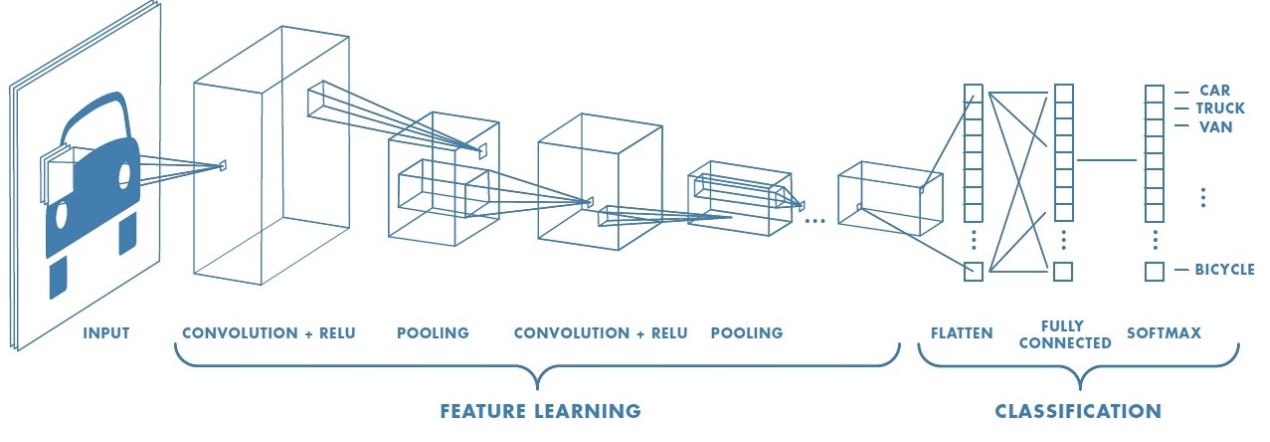
\includegraphics[scale=0.5]{fig5}
    \end{center}
  \caption{CNN Architecture Example}
  \label{fig:CNN}
\end{figure}

\begin{figure}[h!]
  \begin{center}
    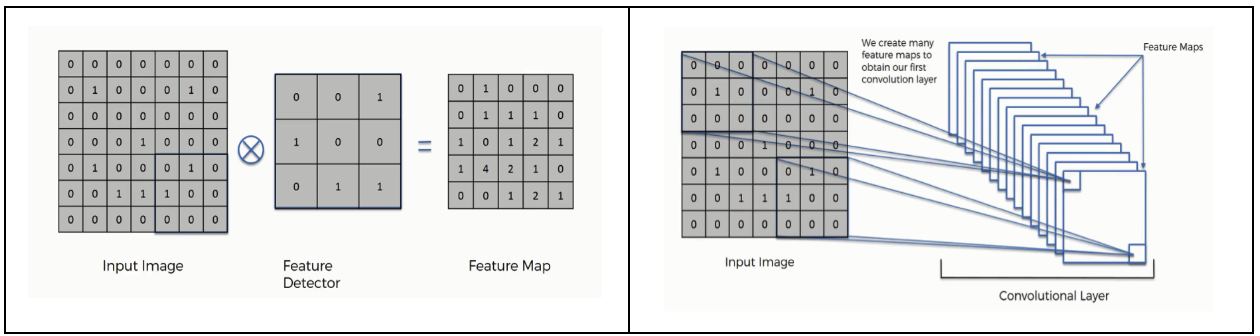
\includegraphics[scale=0.5]{fig6}
    \end{center}
  \caption{Convolution operation with stride=1, padding=None}
  \label{fig:CNNStridePad}
\end{figure}

\begin{figure}[h!]
  \begin{center}
    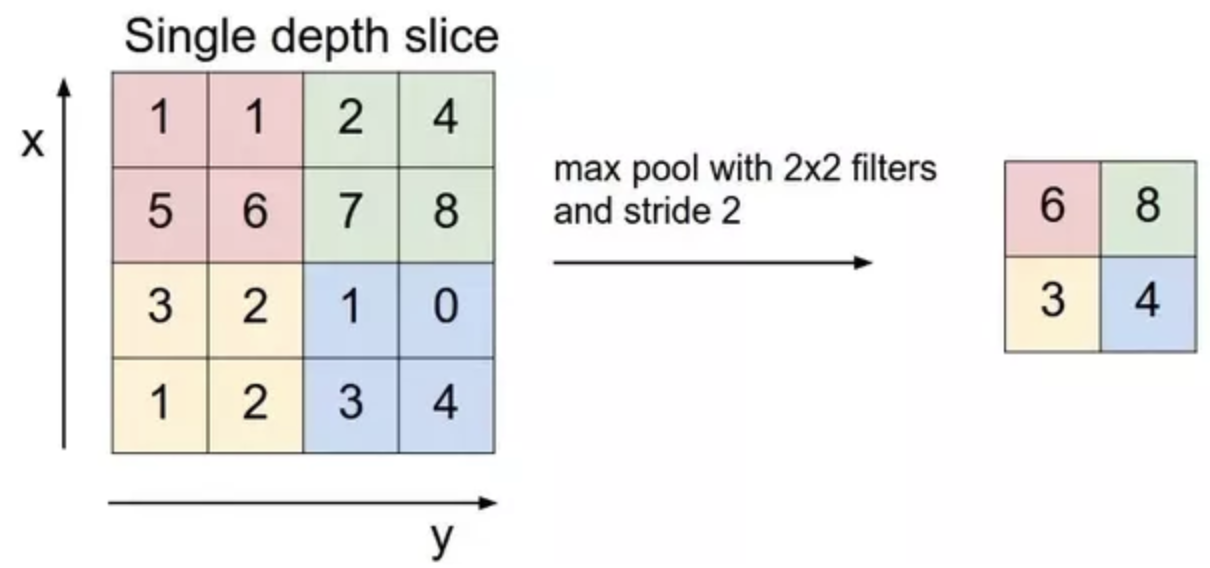
\includegraphics[scale=0.5]{fig7}
  \end{center}
  \caption{Example of Max Pooling}
  \label{fig:CNNPooling}
  \end{figure}

% Fully Connected Neural Network specs

\begin{figure}[h!]
  \begin{center}
    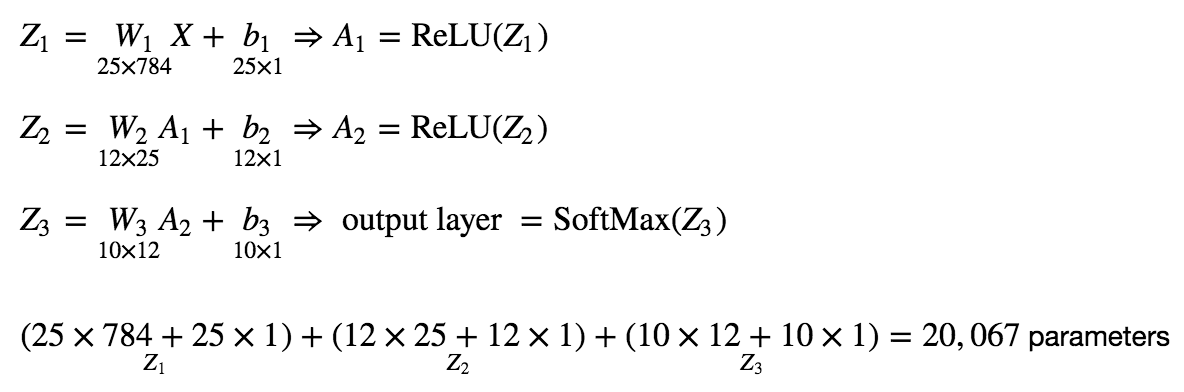
\includegraphics[scale=0.75]{fig2}
    \end{center}
  \caption{Fully Connected Neural Network Architecture}
  \label{fig:fcnn}
\end{figure}

% CNN model specs

\begin{figure}[h!]
  \begin{center}
    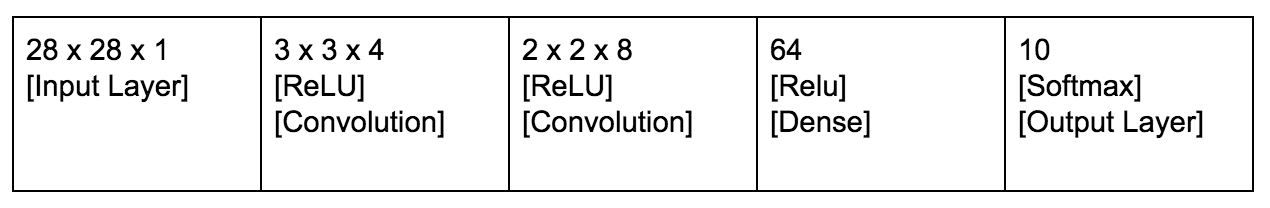
\includegraphics[scale=0.5]{fig3}
    \end{center}
  \caption{(CNN Model 1) Loss Function: Categorical Cross Entropy, Optimizer:
    Adam, Trainable Parameters: 320,890}
  \label{fig:cnnArch}
\end{figure}

\begin{figure}[h!]
  \begin{center}
    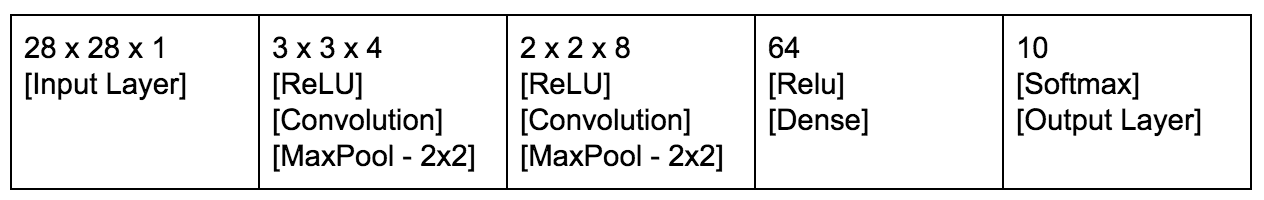
\includegraphics[scale=0.5]{fig4}
  \end{center}
  \caption{(CNN Model 2) Loss Function: Categorical Cross Entropy, Optimizer:
    Adam, Trainable Parameters: 19,322}
  \label{fig:cnnArchPool}
\end{figure}

% H3 results

\begin{figure}[h!]
  \begin{center}
    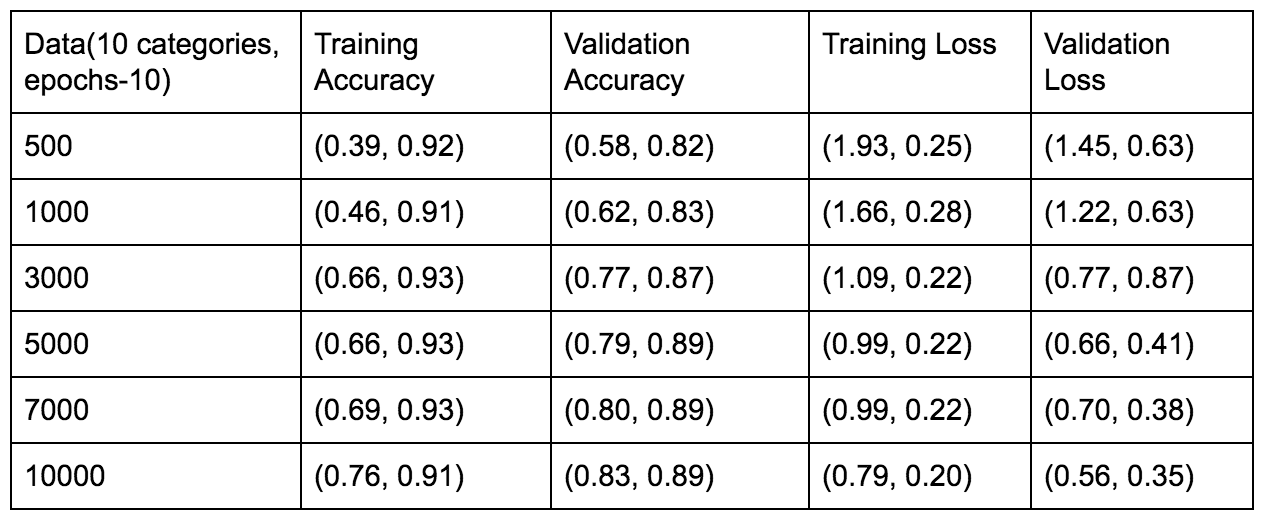
\includegraphics[scale=0.5]{fig8}
    \end{center}
  \caption{$H3_a$ Results for various size training data at (epoch 1,
    epoch 10)}
  \label{fig:h3Results}
  \end{figure}

% H4 results

\begin{figure}[h!]
  \begin{center}
    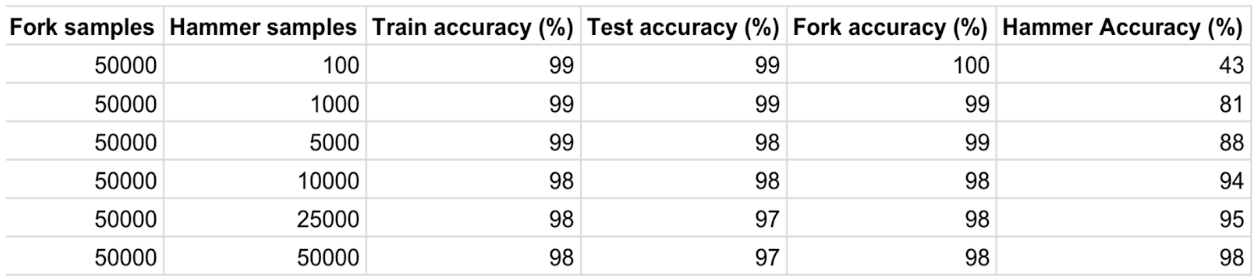
\includegraphics[scale=0.5]{fig9}
    \end{center}
  \caption{$H4_a$ Results for various class imbalances}
  \label{fig:h4Results}
\end{figure}

% H5 results

\begin{figure}[h!]
  \begin{center}
    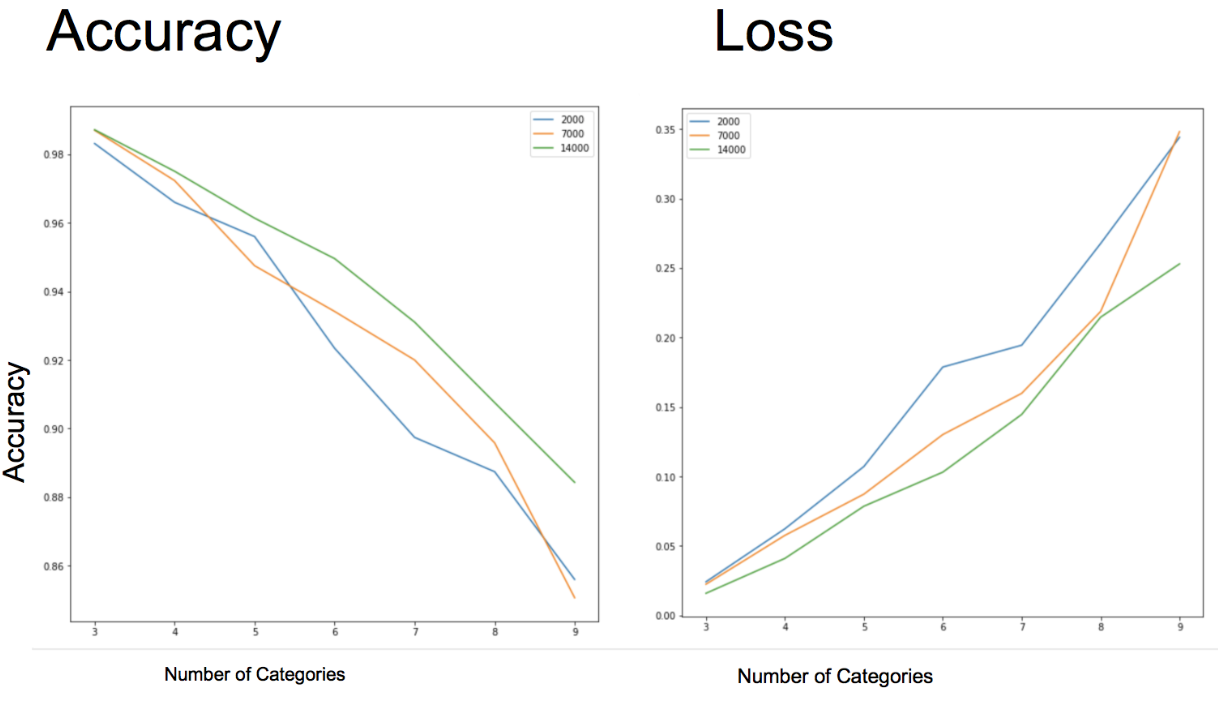
\includegraphics[scale=0.5]{fig10}
    \end{center}
  \caption{$H5_a$ Results for various number of classes $k$}
  \label{fig:h5Results}
\end{figure}

% H6 results

\begin{figure}[h!]
  \begin{center}
    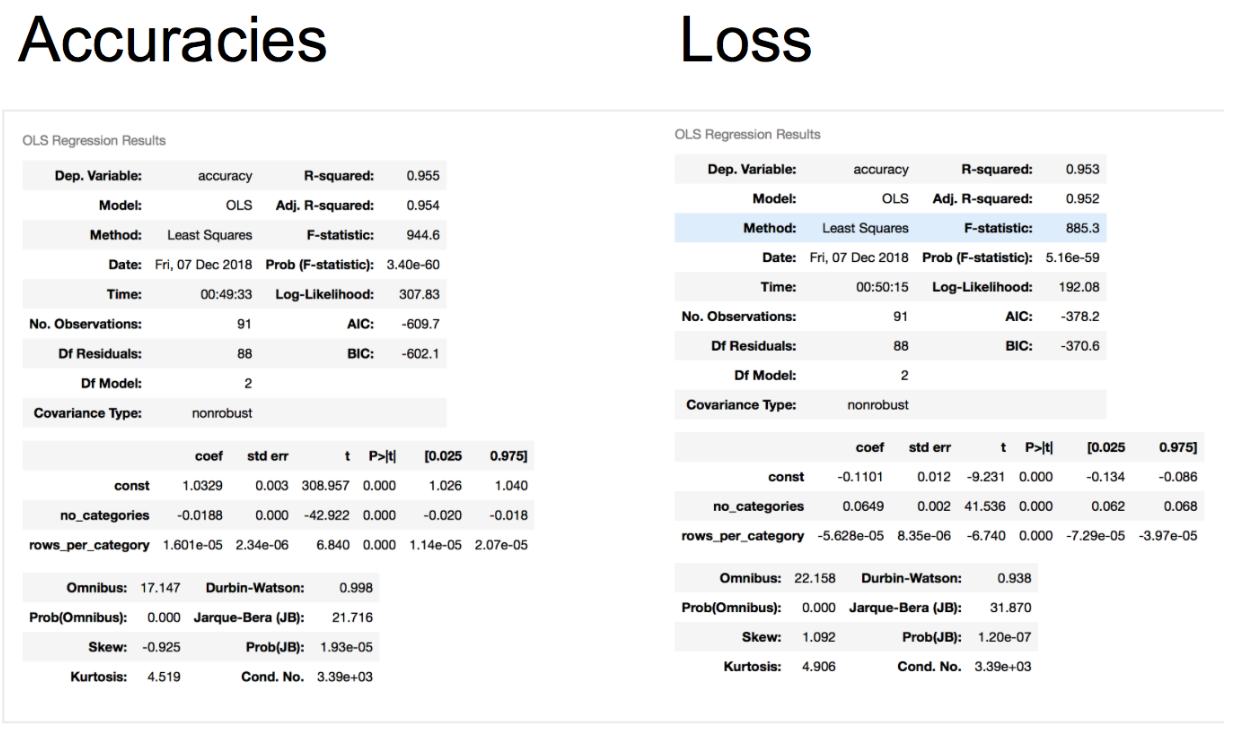
\includegraphics[scale=0.5]{fig11}
    \end{center}
  \caption{$H6_a$ Results for various amounts of training data $n$}
  \label{fig:h6Results}
  \end{figure}





\end{document}
